%auto-ignore
\section{Additional Details for BERT}
\label{appendix:sec:bert_description}



\begin{figure*}[ht]
\begin{center}
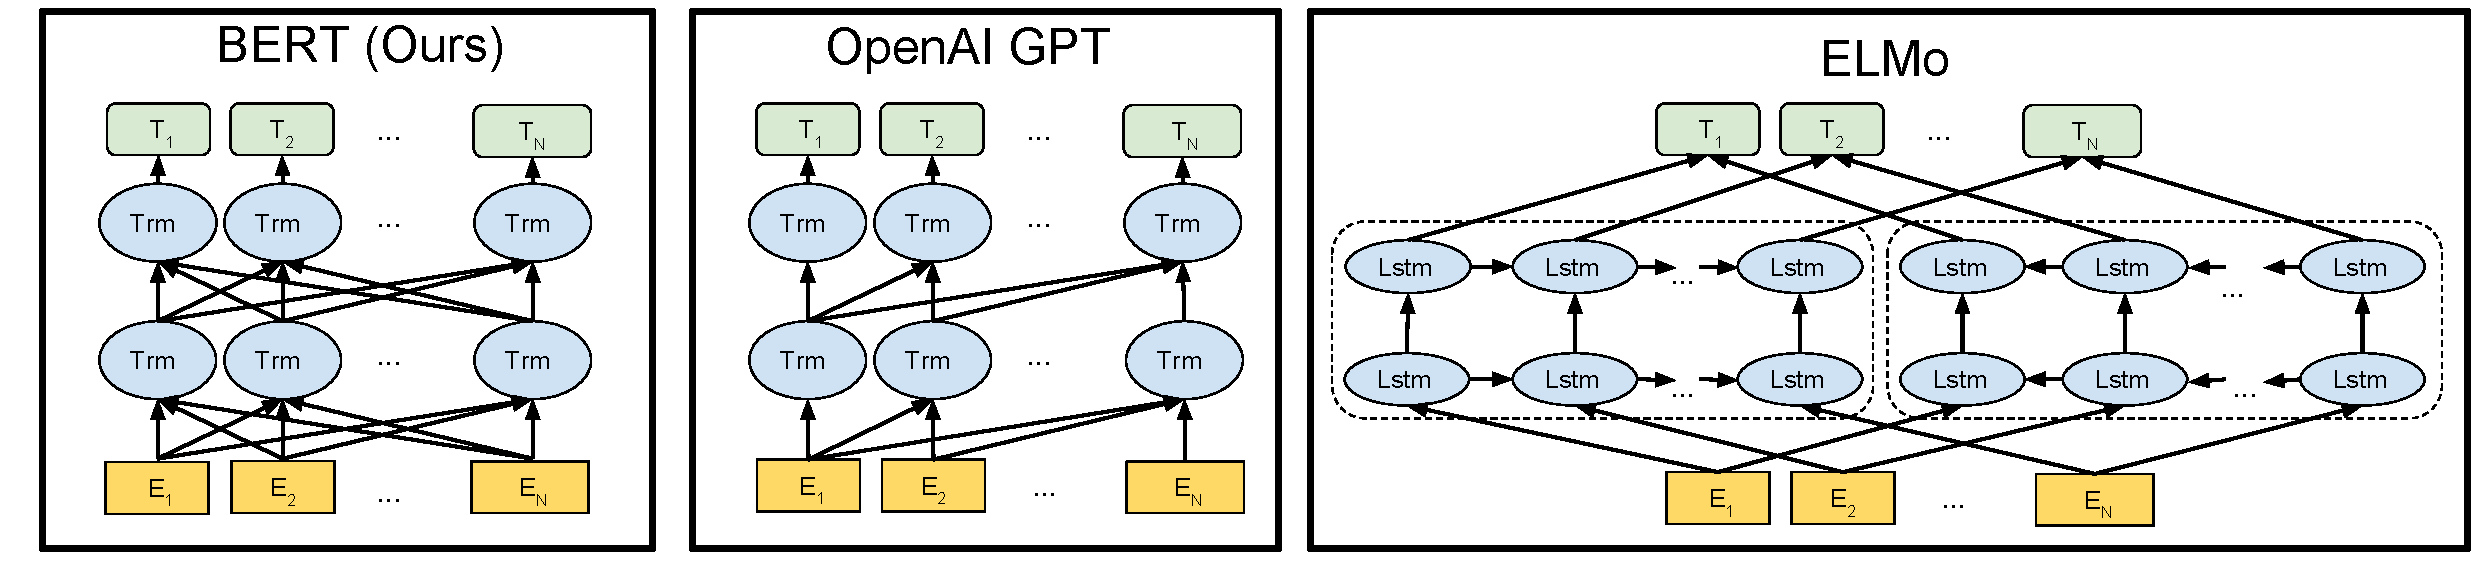
\includegraphics[width=\textwidth]{BERT_comparisons.pdf}
\end{center}
\caption{Differences in pre-training model architectures. BERT uses a bidirectional Transformer. OpenAI GPT uses a left-to-right Transformer. ELMo uses the concatenation of independently trained left-to-right and right-to-left LSTMs to generate features for downstream tasks. Among the three, only \bert representations are jointly conditioned on both left and right context in all layers. In addition to the architecture differences, BERT and OpenAI GPT are fine-tuning approaches, while ELMo is a feature-based approach.}
\label{fig:BERT_comparisons}
\end{figure*}


\subsection{Illustration of the Pre-training Tasks}
We provide examples of the pre-training tasks in the following.

\paragraph{Masked LM and the Masking Procedure} 

Assuming the unlabeled sentence is {\tt {\small my dog is hairy}}, 
and during the random masking procedure we chose the 4-th token (which corresponding to {\tt {\small hairy}}), our masking procedure
can be further illustrated by
\begin{itemize}
%\item Rather than {\em always} replacing the chosen words with {\tt [MASK]}, the data generator will do the following:
\item 80\% of the time: Replace the word with the {\tt [MASK]} token, e.g., {\tt {\small my dog is hairy $\rightarrow$ my dog is [MASK]}}
\item 10\% of the time: Replace the word with a random word, e.g., {\tt {\small my dog is hairy $\rightarrow$ my dog is apple}}
\item 10\% of the time: Keep the word unchanged, e.g., {\tt {\small my dog is hairy $\rightarrow$ my dog is hairy}}. The purpose of this is to bias the representation towards the actual observed word.
\end{itemize}

The advantage of this procedure is that the Transformer encoder does not know which words it will be asked to predict or which have been replaced by random words, so it is forced to keep a distributional contextual representation of {\it every} input token. Additionally, because random replacement only occurs for 1.5\% of all tokens (i.e., 10\% of 15\%), this does not seem to harm the model's language understanding capability. In Section~\ref{appendix:sec:different_masks},
we evaluate the impact this procedure.

Compared to standard langauge model training, the masked LM only
make predictions on 15\% of tokens in each batch, which suggests that more pre-training steps may be required for the model to converge. In Section~\ref{sec:num_training_steps} we demonstrate that MLM does converge marginally slower than a left-to-right model (which predicts every token), but the empirical improvements of the MLM model far outweigh the increased training cost.

\paragraph{Next Sentence Prediction} 

The next sentence prediction task can be illustrated in the following examples.
\begin{align*}
\text{Input\;} &= \text{\tt {\scriptsize [CLS] the man went to [MASK] store [SEP]}} \\ 
& \text{\tt {\scriptsize \;\;\;\;\;\;\;he bought a gallon [MASK] milk [SEP]}}\\
\text{Label} &= \text{\tt {\scriptsize IsNext}} \\
\\
\text{Input\;} &= \text{\tt {\scriptsize [CLS] the man [MASK] to the store [SEP]}}\\
&\text{\tt {\scriptsize \;\;\;\;\;\;\;penguin [MASK] are flight \#\#less birds [SEP]}}\\
\text{Label} &= \text{\tt {\scriptsize NotNext}}
\end{align*}

\subsection{Pre-training Procedure}
\label{sec:pretraining_procedure}

To generate each training input sequence, we sample two spans of text from the corpus, which we refer to as ``sentences'' even though they are typically much longer than single sentences (but can be shorter also). The first sentence receives the {\tt A} embedding and the second receives the {\tt B} embedding. 50\% of the time {\tt B} is the actual next sentence that follows {\tt A} and 50\% of the time it is a random sentence, which is done for the ``next sentence prediction'' task. They are sampled such that the combined length is $\le$ 512 tokens. The LM masking is applied after WordPiece tokenization with a uniform masking rate of 15\%, and no special consideration given to partial word pieces.

We train with batch size of 256 sequences (256 sequences * 512 tokens = 128,000 tokens/batch) for 1,000,000 steps, which is approximately 40 epochs over the 3.3 billion word corpus. We use Adam with learning rate of 1e-4, ${\beta}_1=0.9$, ${\beta}_2=0.999$, L2 weight decay of $0.01$, learning rate warmup over the first 10,000 steps, and linear decay of the learning rate. We use a dropout probability of 0.1 on all layers. We use a {\tt gelu} activation \cite{hendrycks:2016} rather than the standard {\tt relu}, following OpenAI GPT. The training loss is the sum of the mean masked LM likelihood and the mean next sentence prediction likelihood.

Training of \bertbase was performed on 4 Cloud TPUs in Pod configuration (16 TPU chips total).\footnote{https://cloudplatform.googleblog.com/2018/06/Cloud-TPU-now-offers-preemptible-pricing-and-global-availability.html} Training of \bertlarge was performed on 16 Cloud TPUs (64 TPU chips total). Each pre-training took 4 days to complete.

Longer sequences are disproportionately expensive because attention is quadratic to the sequence length. To speed up pretraing in our experiments, we pre-train the model with sequence length of 128 for 90\% of the steps. Then, we train
the rest 10\% of the steps of sequence of 512 to learn the positional embeddings.

\subsection{Fine-tuning Procedure}
For fine-tuning, most model hyperparameters are the same as in pre-training, with the exception of the batch size, learning rate, and number of training epochs. The dropout probability was always kept at 0.1. The optimal hyperparameter values are task-specific, but we found the following range of possible values to work well across all tasks:

\begin{itemize}[noitemsep]
\item {\bf Batch size}: 16, 32
\item {\bf Learning rate (Adam)}: 5e-5, 3e-5, 2e-5
\item {\bf Number of epochs}: 2, 3, 4
\end{itemize}

We also observed that large data sets (e.g., 100k+ labeled training examples) were far less sensitive to hyperparameter choice than small data sets. Fine-tuning is typically very fast, so it is reasonable to simply run an exhaustive search over the above parameters and choose the model that performs best on the development set.

\subsection{Comparison of BERT, ELMo ,and OpenAI GPT}
\label{appendix:sec:comparing_bert_and_openai}

Here we studies the differences in recent popular representation learning
models including ELMo, OpenAI GPT and BERT.
The comparisons between the model
architectures are shown visually in Figure~\ref{fig:BERT_comparisons}. Note that
in addition to the architecture differences, BERT and OpenAI GPT are fine-tuning approaches, while ELMo is a feature-based approach.

The most comparable existing pre-training method to BERT is OpenAI GPT, which trains a left-to-right Transformer LM on a large text corpus. 
In fact, many of the design decisions in BERT were intentionally made to make it as close to GPT as possible so that the two methods could be minimally compared.
The core argument of this work is that the bi-directionality and the two pre-training tasks presented in Section~\ref{sec:pretraining_tasks} account for the majority of the empirical improvements, but we do note that there are several other differences between how BERT and GPT were trained:

\begin{itemize}
\item GPT is trained on the BooksCorpus (800M words); BERT is trained on the BooksCorpus (800M words) and Wikipedia (2,500M words).
\item GPT uses a sentence separator ({\tt [SEP]}) and classifier token ({\tt [CLS]}) which are only introduced at fine-tuning time; BERT learns {\tt [SEP]}, {\tt [CLS]} and sentence {\tt A}/{\tt B} embeddings during pre-training.
\item GPT was trained for 1M steps with a batch size of 32,000 words; BERT was trained for 1M steps with a batch size of 128,000 words.
\item GPT used the same learning rate of 5e-5 for all fine-tuning experiments; BERT chooses a task-specific fine-tuning learning rate which performs the best on the development set.
\end{itemize}

To isolate the effect of these differences, we perform ablation experiments in Section~\ref{sec:task_ablation} which demonstrate that the majority of the improvements are in fact coming from the two pre-training tasks and the bidirectionality they enable.



\subsection{Illustrations of Fine-tuning on Different Tasks}
\label{appendix:sec:fine_tune_details_and_figures}

The illustration of fine-tuning BERT on different tasks can be seen in
Figure~\ref{fig:bert_fine_tune}. Our task-specific models are formed by incorporating \bert with one additional output layer, so a  minimal number of parameters need to be learned from scratch. Among the tasks, (a) and (b) are sequence-level tasks while (c) and (d) are token-level tasks. In the figure, $E$ represents the input embedding, $T_i$ represents the contextual representation of token $i$, \textsc{[CLS]} is the special symbol for classification output, and \textsc{[SEP]} is the special symbol to separate non-consecutive token sequences.
\begin{figure*}[ht]
\begin{center}
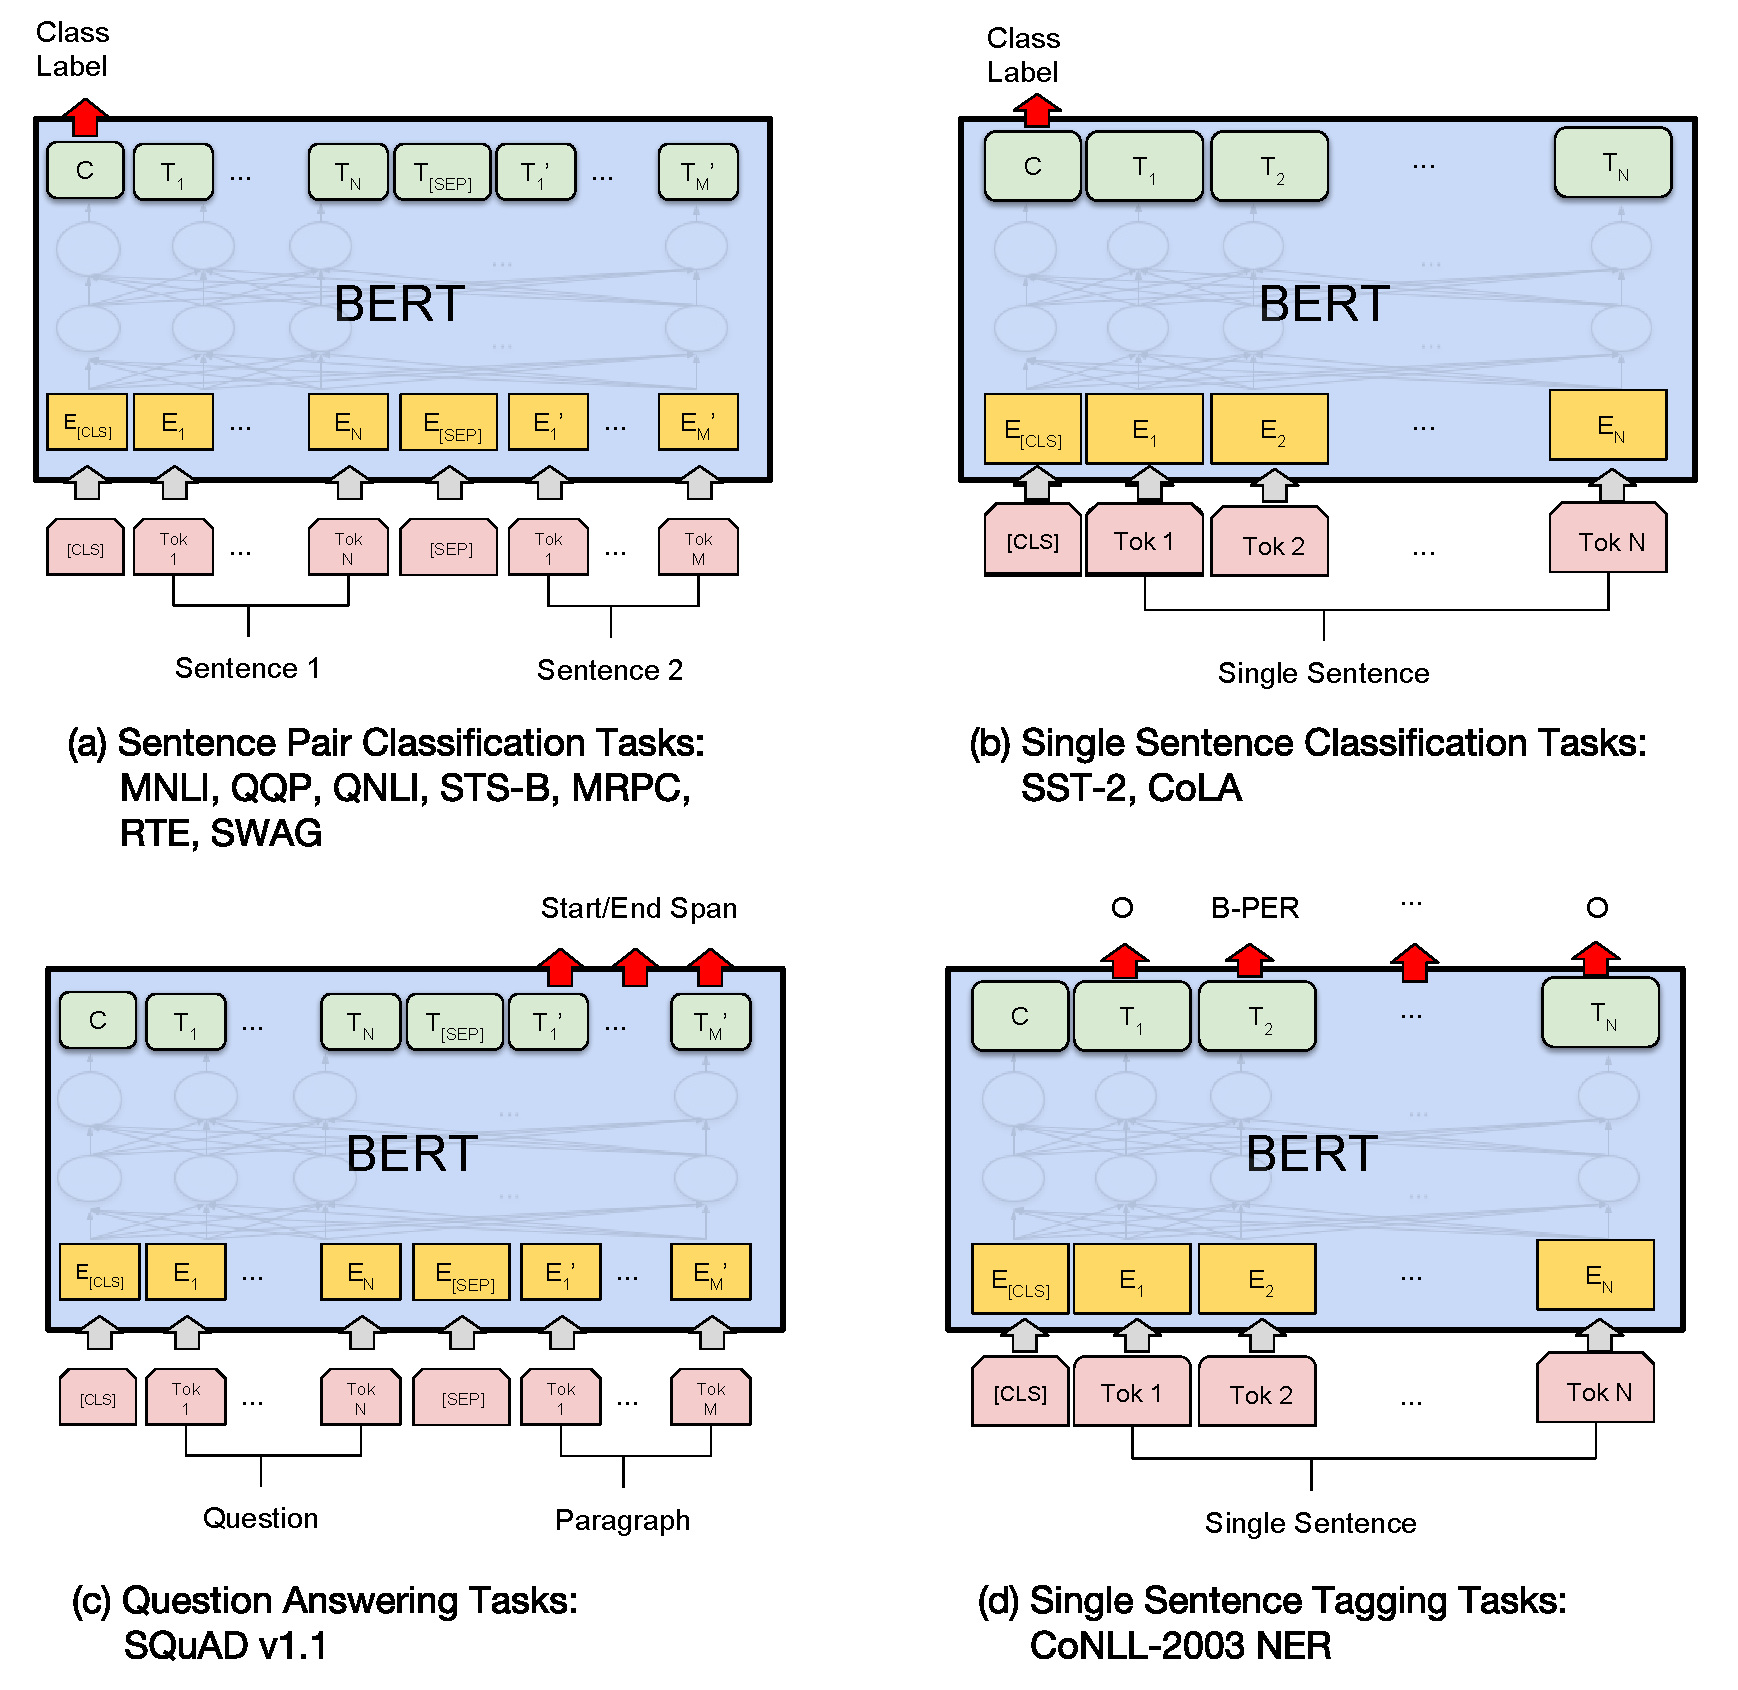
\includegraphics[width=0.85\textwidth]{BERT_fine_tune.pdf}
\end{center}
\caption{Illustrations of Fine-tuning BERT on Different Tasks.}
\label{fig:bert_fine_tune}
\end{figure*}




